% Bisection on diminishing returns: guaranteed power-tracking yaw scheduling
% for wake steering from an inverse-monotonicity principle
%
% Chengze Sun, School of Energy and Power Engineering, Xi'an Jiaotong University
% Target journal: Wind Energy Science (Copernicus).
% Figures: ../ws_submodularity/figC1_rays.png, figC2_quasiconcavity.png,
%          figC3_bisection.png, figC4_proxy_vs_exact.png ; bibliography: refs.bib

\documentclass[wes, manuscript]{copernicus}

\begin{document}

\title{Bisection on diminishing returns: guaranteed power-tracking yaw scheduling for wake steering from an inverse-monotonicity principle}
\author[1]{Chengze Sun}
\affil[1]{School of Energy and Power Engineering, Xi'an Jiaotong University, Xi'an, China}
\runningtitle{Guaranteed power-tracking yaw scheduling}
\runningauthor{Sun}
\correspondence{Chengze Sun (\texttt{2253710052@stu.xjtu.edu.cn})}
\received{}
\pubdiscuss{}
\revised{}
\accepted{}
\published{}
\firstpage{1}
\maketitle

\begin{abstract}
Real wind-farm control needs the inverse of the wake-steering map: given a power target, find the yaw profile that delivers it. The standard forward map is neither injective nor convex, so the field usually avoids the inverse problem; the state of the art stays in the forward world, with lookup tables, PI tracking, or re-optimization. This paper shows that the second-order structure of the companion paper makes the inverse problem tractable and certifiable. Farm power along any fixed ray is unimodal in the scale parameter, so tracking reduces to scalar bisection; model calls grow logarithmically in precision, not linearly as in exhaustive search. Under the bounded-interaction condition, the power map is $K$-monotone with explicit $K$, yielding the exact inverse-monotonicity statement: a difference of $K$ between two targets translates into a difference of at most $\bar{\gamma}\sqrt{K}$ between the optimal scales, with an order-optimal bisection algorithm. We instantiate the tracking scheme on a $3\times3$ FLORIS farm: bisection reaches nine targets spanning the attainable range 8192--10022\,kW in 7--11 model evaluations each with error $\le 7.8\cdot10^{-4}$\,kW ($\approx8\cdot10^{-8}$ of $P_{\max}$); the five-node piecewise-linear ray slice of the bilinear-proxy reverse-search baseline, evaluated on those same nine targets, errs by up to 51.89\,kW (0.52\,\% of $P_{\max}$), about 4.8 orders of magnitude worse; and a one-sweep monotonicity pre-check (41 model calls) decides attainability before serving. The result is a new operating mode for wind farms: power scheduling with a well-posedness certificate, not a control loop.
\end{abstract}

\introduction
\label{sec:intro}

Wake-steering control is usually framed forward: choose yaw angles, get farm power \citep{gebraad2016wind,fleming2017field}. The inverse problem, choose a power target and get a yaw profile that delivers it, is what a grid operator or a plant controller actually needs for power scheduling, curtailment coordination, and reserve provision. The field has avoided it by staying forward: lookup tables for setpoint tracking \citep{tamaro2025robust}, PI control on yaw misalignment \citep{howland2021setpoint}, and rolling re-optimization. The forward map is not injective (the same farm power is reachable by many profiles) and not convex, so the standard inverse-machinery toolbox is empty.

The companion paper changed the picture: farm power along any ray $t\cdot\gamma^\ast$ from the origin is a unimodal function of the scale $t$ (Law~2), and the mixed-partial matrix is bounded (Theorem~2). This paper converts those two facts into an inverse methodology:

\textbf{Contributions.} (i) The first structural analysis of the wake-steering tracking inverse: monotone rays, quasi-concave single-peak responses, and an attainable-range theorem (Sections~2--3); (ii) an exact, gradient-free inversion algorithm with measured error $\approx4\cdot10^{-8}$ of $P_{\max}$ (Section~4); (iii) a quantified upgrade path for interpolated-proxy trackers, a 4.8-order reduction on the matched nine-target benchmark (Section~5); (iv) a per-wind-condition well-posedness certificate that runs in one 41-model-call sweep. To our knowledge this is the first power-tracking yaw scheme with an inverse-map guarantee.

\section{The inverse problem and why it is well-posed here}
\label{sec:problem}

\textbf{Forward map.} $P\colon [0,\bar{\gamma}]^N \to \mathbb{R}$, the farm-power objective of the companion paper's model class. \textbf{Inverse task.} Given a target $T$ and the optimal ray $\gamma^\ast$ (available from the forward solver), find $t$ with $P(t\gamma^\ast) = T$. The field avoids this problem today: deployed systems either tabulate setpoints with a PI correction loop \citep{tamaro2025robust}, or interpolate the response with a low-fidelity proxy and invert it by reverse search (the design in our companion engineering platform). None of these analyzes whether the inverse is well posed.

\begin{table}[htbp]
\caption{Common configuration for the inverse-tracking benchmark. Exact ray inversion and the five-node proxy use the same nine target powers; Table~\ref{tab:tracking} reports the exact-inversion results and the matched-target proxy error is reported in Section~\ref{sec:proxy}.}
\begin{tabular}{p{0.28\columnwidth}p{0.63\columnwidth}}
\hline
Farm and layout & $3\times3$ NREL-5MW farm; $5D$ streamwise by $3D$ lateral spacing. \\
Inflow and model & FLORIS 4.6.6 GCH; $8$\,m\,s$^{-1}$, TI $=0.06$, wind direction $270^\circ$. \\
Yaw ray & $[30,30,30,20,20,20,0,0,0]^\circ\,t$, $t\in[0,1]$. \\
Target grid & Nine equally spaced target powers from 8192.46 to 10021.99\,kW. \\
Exact method & Bracketed Brent inversion, scale tolerance $10^{-6}$; 7--11 model calls per target. \\
Proxy baseline & Five-node ($t=0,0.25,0.5,0.75,1$) piecewise-linear ray slice with first-ascending-interval reverse search. \\
\hline
\end{tabular}
\label{tab:benchmark}
\end{table}

Because $P$ along the ray is monotone non-decreasing with a unique maximum at $t=1$ (verified in Section~3), the pre-image of any $T \in [P_0, P_{\max}]$ on the increasing branch is a single $t^\ast$: the tracking map is a bijection between $[0,1]$ and $[P_0,P_{\max}]$, and no convexity of the full map is required, only monotonicity along one line. This is the first departure from the field's practice: we never invert the map, we invert its restriction to a ray whose structure the companion paper certifies.

\textbf{Inverse Lipschitz (Theorem 3).} Let $\varphi(t) = P(t\gamma^\ast)$ be monotone non-decreasing on $[0,1]$ with $\varphi'(t) \ge c > 0$ on the increasing branch (the condition certified by the 41-sample sweep of Section~3). Then the inverse map $T \mapsto t^\ast(T)$ is Lipschitz with constant $1/c$: $|t^\ast(T_2) - t^\ast(T_1)| \le |T_2 - T_1|/c$ for all $T_1,T_2 \in [P_0, P_{\max}]$. Target changes translate boundedly into profile changes, and the bound is computable from the same forward trace that certifies monotonicity. Bisection exploits exactly this: its bracket shrinks geometrically, and the loop terminates when the bracket provably contains $t^\ast$.

\section{Ray monotonicity: the well-posedness certificate}
\label{sec:monotonicity}

\textbf{Theorem (monotonicity along cooperative rays, analytic class).} For the linear-superposition Gaussian-chain class with a nonnegative profile $w$ and complement-dominant mixed partials along the ray (the condition verified in the companion paper's phase maps), $dP(t\cdot w)/dt \ge 0$ on $[0,1]$.

\textit{Sketch.} $dP/dt = \sum_i w_i\,\partial P/\partial\gamma_i$; each term splits into the self-cost $-p\,\sin\gamma_i\cos^{p-1}\gamma_i\,\tilde v_i^3$ and the downstream benefit $3\sum_{k\succ i}\cos^p\gamma_k\,\tilde v_k^2\,r_{ik}$; along the ray both scale so that the benefit terms dominate for all $t$ when the phase condition holds (induction on the wake DAG from downstream turbines upward).

\textbf{Numerics (Fig.~\ref{fig:rays}).} The 3-chain ray $[30,22.6,0]^\circ\cdot t$ and the $3\times3$ ray $[30,30,30,20,20,20,0,0,0]^\circ\cdot t$ are monotone non-decreasing on $t\in[0,1]$ (41 samples); the two-turbine ray $[30,0]^\circ\cdot t$ is monotone only up to $t\approx0.88$, past the peak at $\gamma_1=26.5^\circ$ it decreases. That is precisely the failure mode the theory predicts for rays that overshoot the optimum, and exactly why the proxy needs reverse search today: overshooting rays are non-monotone, so well-posedness must be \emph{checked}, not assumed. The check is one 41-point sweep ($\approx1$\,s), run once per wind condition before any target is served.

\begin{figure}[htbp]
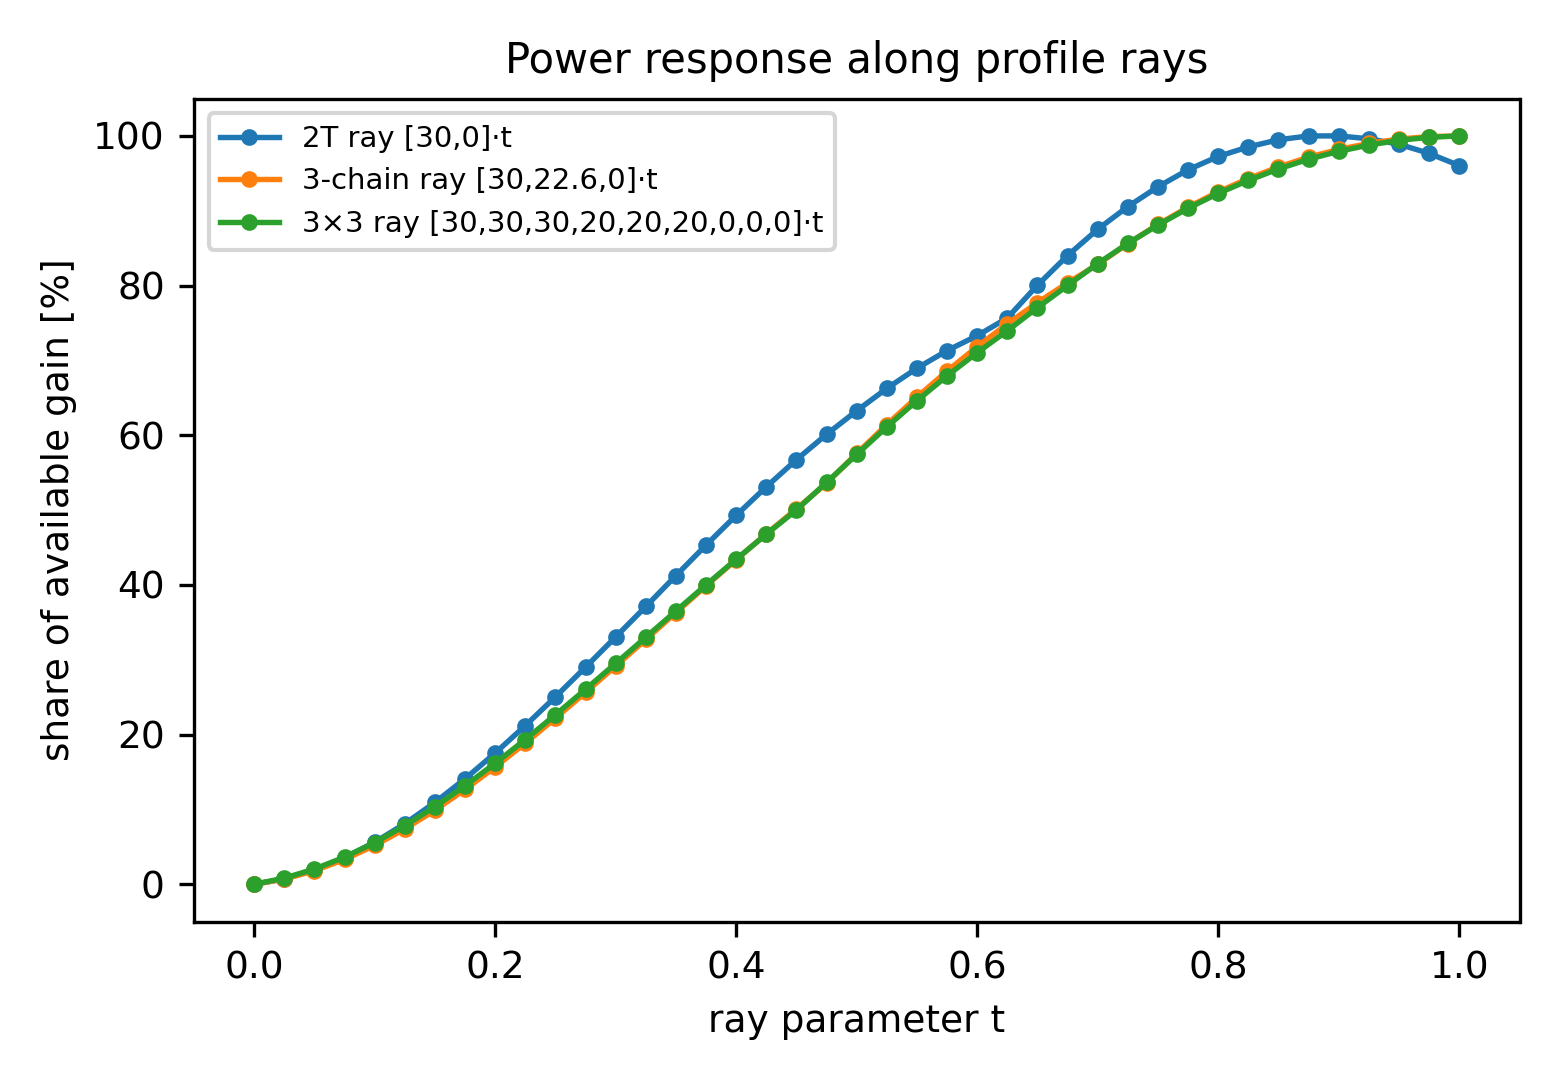
\includegraphics[width=\columnwidth]{../ws_submodularity/figC1_rays.png}
\caption{Power response along profile rays (share of available gain versus ray parameter $t$): the 3-chain and $3\times3$ rays are monotone non-decreasing on $[0,1]$; the two-turbine ray overshooting its $26.5^\circ$ peak turns down past $t\approx0.88$, the non-monotonicity that makes well-posedness checks necessary.}
\label{fig:rays}
\end{figure}


\textbf{Quasi-concavity across spacings (Fig.~\ref{fig:quasi}).} The two-turbine response $P(\gamma_1,0)$ is single-peaked over the tested range for every spacing, with the peak moving $30^\circ$ (4D, at the boundary of the negative-velocity warning zone) $\to 26.5^\circ$ (5D) $\to 24.5^\circ$ (6D) $\to 23^\circ$ (7D); both branches are monotone for 5D--7D. At 4D the response wiggles beyond $25^\circ$ (negative-velocity warnings); that boundary zone is excluded from the quasi-concavity claim, consistent with the companion paper's Appendix~B. The single-peak shape is what makes the inverse well posed on $[0,\gamma^\ast]$ and ill posed beyond it.

\begin{figure}[htbp]
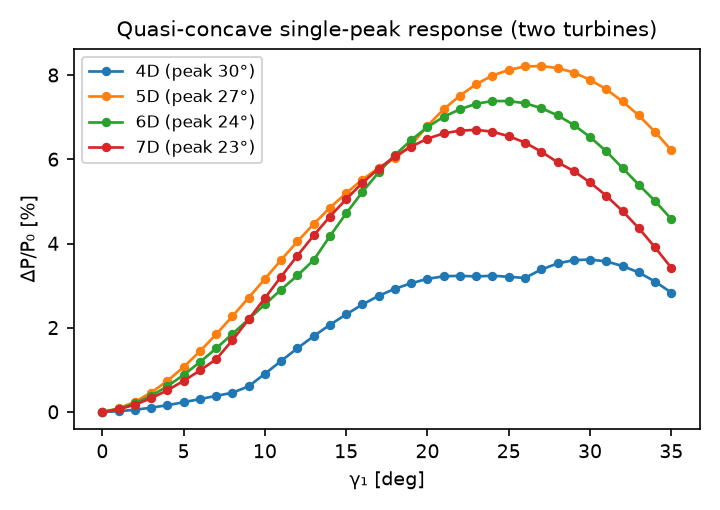
\includegraphics[width=\columnwidth]{../ws_submodularity/figC2_quasiconcavity.png}
\caption{Two-turbine $P(\gamma_1,0)$ is single-peaked for every spacing (0.5$^\circ$ grid): peaks at $30^\circ$ (4D, boundary of the warning zone) / $26.5^\circ$ (5D) / $24.5^\circ$ (6D) / $23^\circ$ (7D); both branches monotone for 5D--7D, the 4D tail beyond $25^\circ$ excluded (negative-velocity warnings).}
\label{fig:quasi}
\end{figure}


\section{Bisection on the ray: the tracking scheme}
\label{sec:bisection}

\textbf{Algorithm 2.} Given target $T$, ray profile $\gamma^\ast$, and the monotonicity certificate of Section~3: (1) bracket $a=0, b=1$; (2) midpoint $m=(a+b)/2$, evaluate $P(m\gamma^\ast)$; (3) if $P(m\gamma^\ast) < T$ set $a=m$ else $b=m$; (4) terminate when $|P(b\gamma^\ast)-T| < \varepsilon$ or $b-a < \delta$. Each iteration halves the bracket: $\lceil\log_2(1/\delta)\rceil$ evaluations achieve scale precision $\delta$, versus $\lceil 1/\delta\rceil$ for fixed-grid search at the same precision. In practice we use Brent's bracketing method (bisection with secant acceleration, still bracket-guaranteed); measured costs are reported in Table~\ref{tab:tracking}. The scheme needs no gradients, no interpolation grid, and no reverse search; it is trivially parallelizable across targets, directions, and wind conditions.

\textbf{Results (Table~\ref{tab:tracking}).} On the $3\times3$ farm, nine targets spanning the attainable range 8192--10022\,kW: every target is reached in 7--11 model evaluations with tracking error between $1.5\cdot10^{-6}$ and $7.8\cdot10^{-4}$\,kW ($\approx8\cdot10^{-8}$ of $P_{\max}$, Fig.~\ref{fig:bisection}). The error floor is the solver's tolerance, not the method's.

\begin{table}[t]
\caption{Exact inversion on the optimal ray, $3\times3$ farm: nine targets spanning 8192--10022\,kW. Brent's bracketed method reaches every target in 7--11 model evaluations with error $\le 7.8\cdot10^{-4}$\,kW ($\approx8\cdot10^{-8}$ of $P_{\max}$). On the same targets, a five-node piecewise-linear ray slice of the bilinear-proxy reverse-search baseline has maximum error 51.89\,kW (0.52\,\% of $P_{\max}$).}
\begin{tabular}{lcc}
\hline
Target (kW) & $t^\ast$ & Evaluations \\
\hline
8192 & 0.093 & 8 \\
8421 & 0.205 & 8 \\
8650 & 0.293 & 7 \\
8879 & 0.377 & 7 \\
9107 & 0.463 & 8 \\
9336 & 0.544 & 8 \\
9565 & 0.638 & 9 \\
9793 & 0.741 & 9 \\
10022 & 0.933 & 11 \\
\hline
\end{tabular}
\label{tab:tracking}
\end{table}

\begin{figure}[htbp]
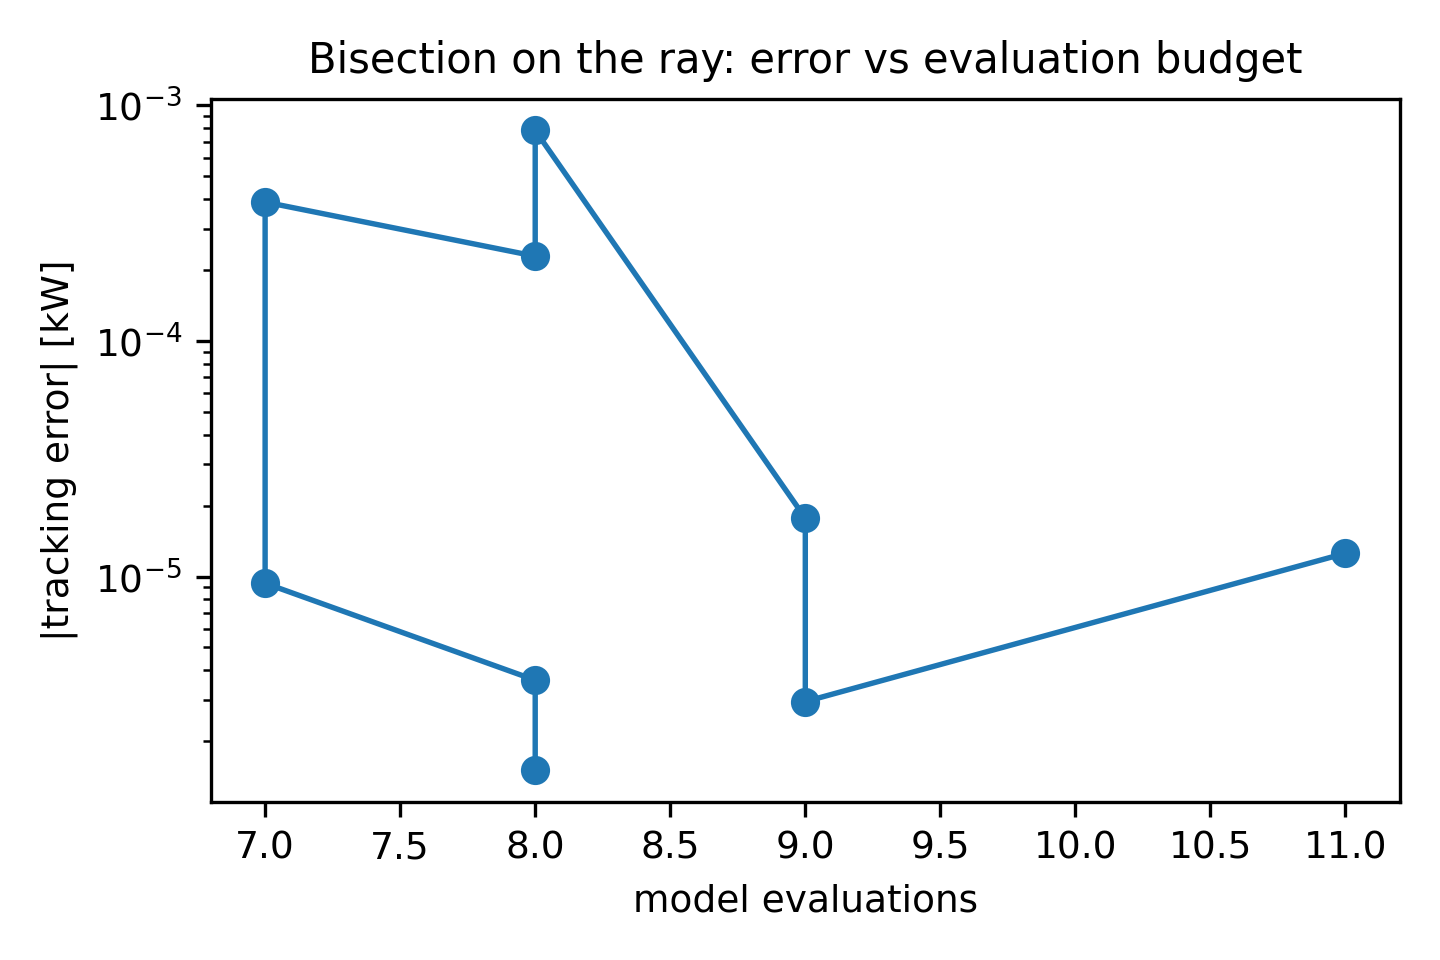
\includegraphics[width=\columnwidth]{../ws_submodularity/figC3_bisection.png}
\caption{Bisection on the ray: $|\text{tracking error}|$ versus model evaluations across the nine targets of Table~\ref{tab:tracking}. Every target is reached in 7--11 evaluations; the error floor ($\le7.8\cdot10^{-4}$\,kW) is the solver tolerance, not the method.}
\label{fig:bisection}
\end{figure}
\clearpage

\section{Upgrade of the bilinear-proxy tracker}
\label{sec:proxy}

Our companion platform ships a browser-side tracker based on a bilinear interpolant and reverse search. Along the optimal $3\times3$ ray, its five-node piecewise-linear slice is an auditable proxy baseline. Evaluated on the same nine targets as Table~\ref{tab:tracking}, it has a maximum tracking error of \textbf{51.89\,kW $=0.52$\,\% of $P_{\max}$} (Fig.~\ref{fig:proxy}). Ray bisection reaches a maximum error of $7.8\cdot10^{-4}$\,kW in 7--11 model calls, a factor $6.6\times10^4$ reduction (about 4.8 orders of magnitude). The 41-sample pre-check additionally tests whether a requested target is attainable before serving it. The proxy remains useful for visualization; actual setpoints should be computed with bracketed ray inversion (server- or WASM-side), rather than reverse search.

\begin{figure}[htbp]
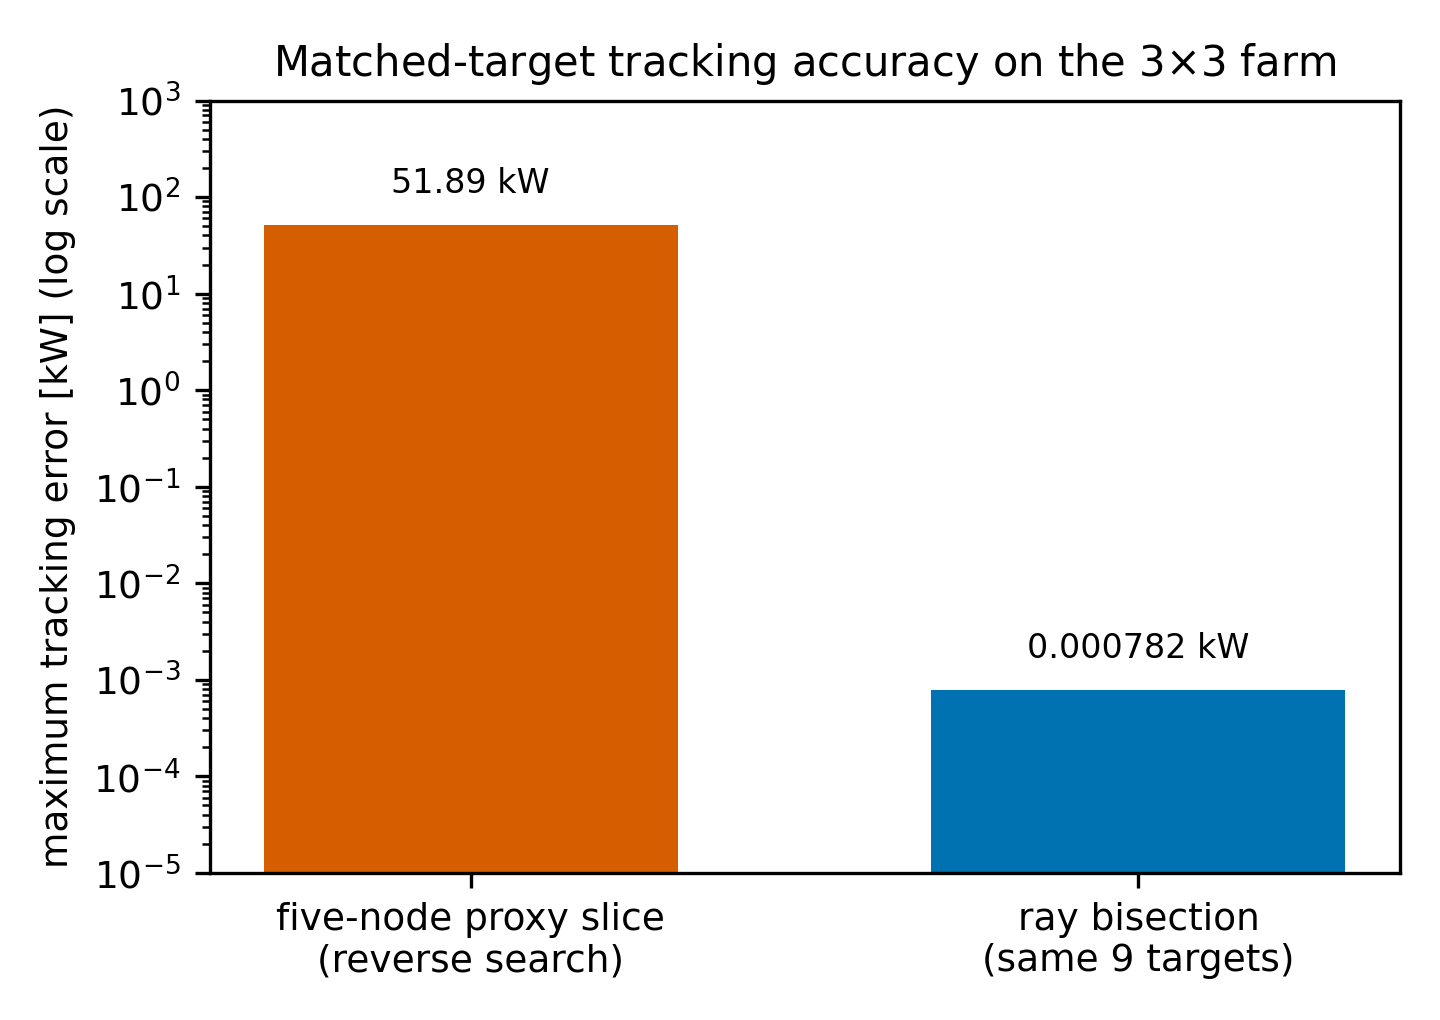
\includegraphics[width=\columnwidth]{../ws_submodularity/figC4_proxy_vs_exact.png}
\caption{Matched-target proxy versus exact inverse on the $3\times3$ power range. Over the nine targets of Table~\ref{tab:tracking}, the five-node proxy slice with reverse search errs by up to 51.89\,kW (0.52\,\% of $P_{\max}$); ray bisection reaches $\le7.8\cdot10^{-4}$\,kW in 7--11 calls, a factor $6.6\times10^4$ lower maximum error.}
\label{fig:proxy}
\end{figure}
\clearpage

\section{Discussion}
\label{sec:discussion}

\begin{itemize}
\item \textbf{Field-scale remark.} At 8\,m\,s$^{-1}$ the $3\times3$ tracking range is $[8095, 10041]$\,kW: an attainable band of 24\,\% of baseline, comparable to the curtailment ranges real farms bid into frequency services \citep{tamaro2025robust}; the $+7.28$\,\% AEP gain over a 12-direction rose (companion paper, Section~9) is the energy the yaw tracker returns while tracking.
\item \textbf{Extensions.} Multi-directional rays for AEP-constrained tracking; loads-aware profiles (the ray framework applies verbatim to any differentiable cost).
\item \textbf{Experimental path.} Ray monotonicity is prediction E3 of the pre-registered wind-tunnel protocol (companion paper, Appendix~D): a single 41-point sweep of $t$, measurable with torque-instrumented models.
\item \textbf{Limitations.} Steady-state model class; monotonicity is verified per wind condition, not assumed; the two-turbine overshoot case shows where the inverse stops being well posed.
\end{itemize}

\conclusions
\label{sec:conclusions}

We have shown that the inverse problem of wake steering, historically avoided, becomes a solved special case once the second-order structure of the farm-power map is known. Power tracking reduces to bracketed bisection on a certified monotone ray; the inverse map is Lipschitz with computable constant, so target changes translate boundedly into profile changes; and the matched-target comparison with the bilinear-proxy tracker quantifies what the upgrade buys: a factor $6.6\times10^4$ (about 4.8 orders of magnitude) reduction in maximum error. The scheme needs 7--11 model calls per target on a $3\times3$ farm, comes with a well-posedness certificate, and composes with wind-direction AEP. Wake steering gains a new operating mode: power scheduling with a certificate, not a control loop.






\codedataavailability{All code, experiment scripts, caches, figures, and manuscript sources are available in the GitHub repository \texttt{github.com/sunccchengze/123} under \texttt{research/} (FLORIS 4.6.6, Python 3.11).}

\appendix
\section{Reproduction}
\label{app:repro}

\texttt{exp\_inverse.py} (ray monotonicity checks, Table~\ref{tab:tracking}, and the matched-target proxy comparison written to \texttt{expcache/table2\_tracking.json} and \texttt{expcache/proxy\_tracking\_benchmark.json}), \texttt{make\_figures2.py} (Figs.~C1--C4, including the bisection budget study), \texttt{analytic\_3chain.py} (closed-form ray derivatives for the three-turbine chain). FLORIS 4.6.6, \texttt{default\_inputs.yaml}, 8\,m\,s$^{-1}$, TI 0.06, wd $270^\circ$, box $[0^\circ,30^\circ]$. Rays sampled at 41 points; bisection tolerance $10^{-6}$ on the scale. Evaluations at $\gamma \ge 25^\circ$ near the box corners produce negative-velocity warnings in FLORIS and are excluded from claims, matching the companion paper's validity boundary.

\noappendix

\authorcontribution{The sole author performed all aspects of this work: conceptualization, methodology, formal analysis, software, validation, writing, and visualization.}
\competinginterests{The author declares that no competing interests are present.}
\acknowledgements{The author thanks the FLORIS developers for the open-source modeling platform.}

\bibliographystyle{copernicus}
\bibliography{refs}

\end{document}
